% This is a LaTeX driving document to produce a standalone copy
% of the project proposal held in propbody.tex.  Notice that
% propbody can be used in this context as well as being incorporated
% in the dissertation (see diss.tex).
\documentclass[a4 paper,twoside,12pt]{article}
\usepackage{verbatim}
\usepackage{hyperref}
\usepackage[scale=0.825]{geometry}
\usepackage{graphicx}

\parindent 0pt
\parskip 6pt

\begin{document}

\pagenumbering{gobble}

\begin{titlepage}

\rightline{\large\emph{Thomas Lefley}}
\medskip
\rightline{\large\emph{Girton College}}
\medskip
\rightline{\large\emph{tl364}}

\vfil
\centerline{\large Computer Science Part II Project Proposal}
\vspace{0.4in}
\begin{center}
\Large\bf Mesh to voxel transformation for optimised physics-based interactions
\end{center}
\vspace{0.3in}
\centerline{\large \emph{24/10/2014}}

\vfil

\eject

\end{titlepage}

\cleardoublepage

\pagenumbering{arabic}

%!TEX root = Lefley - Mesh to voxel transformations for optimised physics-based interactions.tex
\chapter{Introduction}

\section{Motivation}

Physics simulation is one of the key components of a modern game engine. The more accurate the simulation is, the more immersive games built with the engine are likely to be. If the world around the player does not react as expected then it is difficult to become immersed in the game environment.

\section{Problem}

\label{sect:prob}

The most common representation of a solid object in a physical simulation is a rigid polygonal mesh. This format stores the vertices and faces which define the object's surface, with volume information being implicit. This is optimal for operations which require only the surface information, such as rendering, but presents issues if we wish to reason on the object's interior, as we do when fragmenting under physical forces.

It is possible to fragment an object without knowledge of its interior by simply partitioning the space in which the object exists and refining any partitions which have faces in them. However, as no volumetric information about the object is being used, the fracturing is approximate. A further limitation is that most implementations using similar approaches are restricted to convex objects or must first decompose any concave objects into constituent convex meshes~\cite{Muller:2013:RTD:2461912.2461934}.

Overall, while fragmentation from only surface information is efficient and produces reasonable results, the physical accuracy is limited and this project instead proposes a method which uses the object's volumetric information.

\section{Solution}

\label{sect:sol}

Taking an object as a three dimensional scalar field of mass, we simplify the problem of fragmenting it on the applied physical forces. For each point inside the object we determine which fragment that point should belong to based on the object's physical properties.

When only the boundary is stored, determining whether any given point is inside of an object is non trivial. Consider a series of faces defining a 2D object. Then to label any given point as inside the object we need to check that it is `inside' of all of the faces\cite{Ray-tracing}. Furthermore, this only holds for convex shapes, if there exist any concave sections then we could have a point which is `outside' of a face but inside the 2D object. See Figure~\ref{fig:1.1}.

\begin{figure}[b!]
\centerline{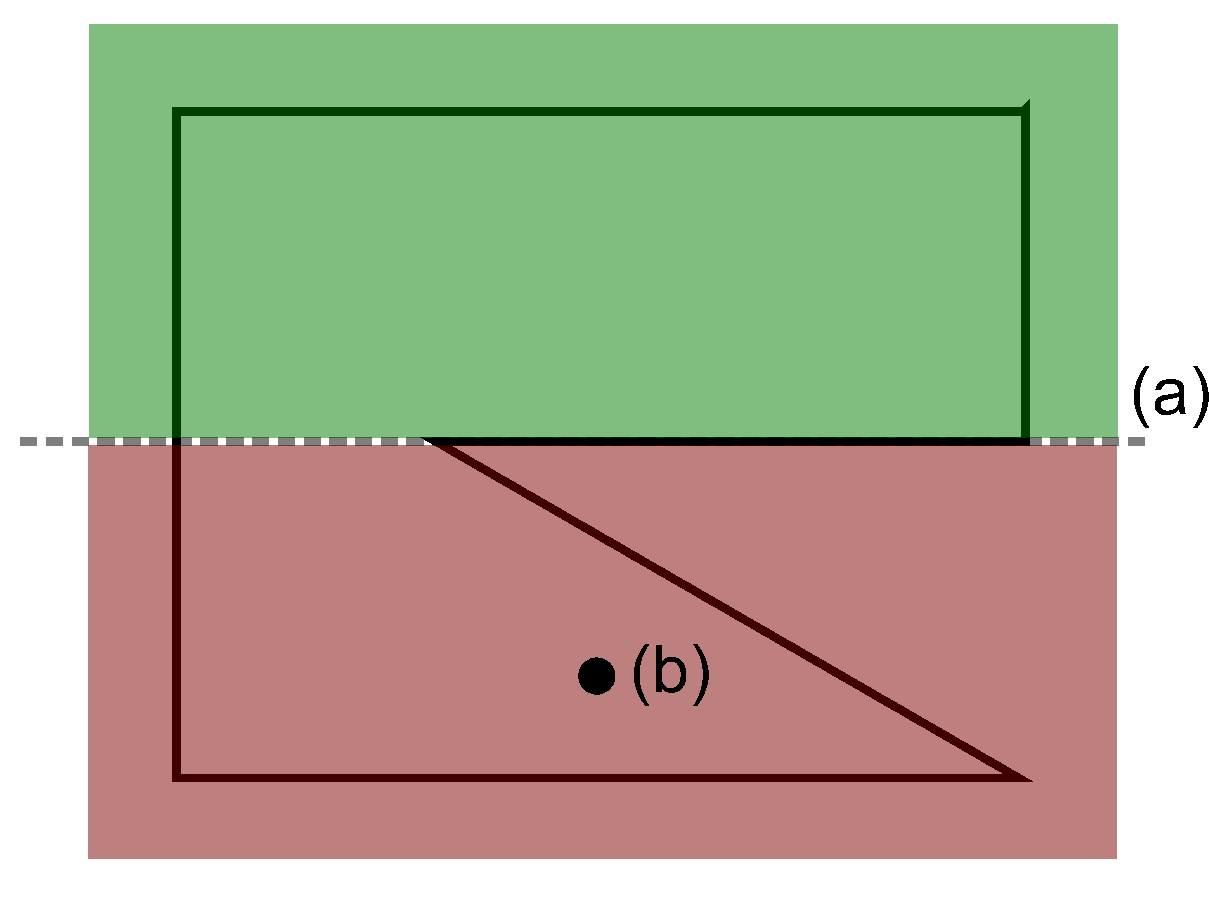
\includegraphics[scale=0.4]{point_inside_concave13.pdf}}
\caption{The green area shows all points `inside' line (a). The red areas shows all points `outside' line (a). Point (b) is `outside' line (a) but inside the defined concave shape.}
\label{fig:1.1}
\end{figure}

Calculating for all points, whether they are inside the object before physical interaction can reduce the simulation time complexity discussed above. We also gain a constant time lookup for checking if any given point lies within the object. This process is known as binary solid voxelisation, where a binary voxel is a point in three dimensional space with an assignment based on whether it is inside or outside of a given object\cite{Schwarz:2010:Vox}.

This project proposes a pipeline for simulating physical destruction, focussing on fragmentation, consisting of the following stages.
\begin{enumerate}
\item{Objects are voxelised}
\item{Each voxel is assigned to a fragment algorithmically in such a way as to emulate the physical properties of the object}
\item{A rigid mesh is built for each fragment from its constituent voxels}
\end{enumerate}

For example, if a bullet is fired at a brick wall, both the bullet and wall will be rigid meshes when the bullet is shot. On collision, both the wall and bullet will be voxelised. Assuming the bullet consists of only one voxel, no destruction calculations will be performed on it. Using the force of impact and physical parameters of the wall, it will be calculated which voxels should belong to which fragments. These fragments will then be transformed back into rigid meshes and the correct movement vectors will be applied. This is illustrated in Figure~\ref{fig:1.2}.

\begin{figure}
\centerline{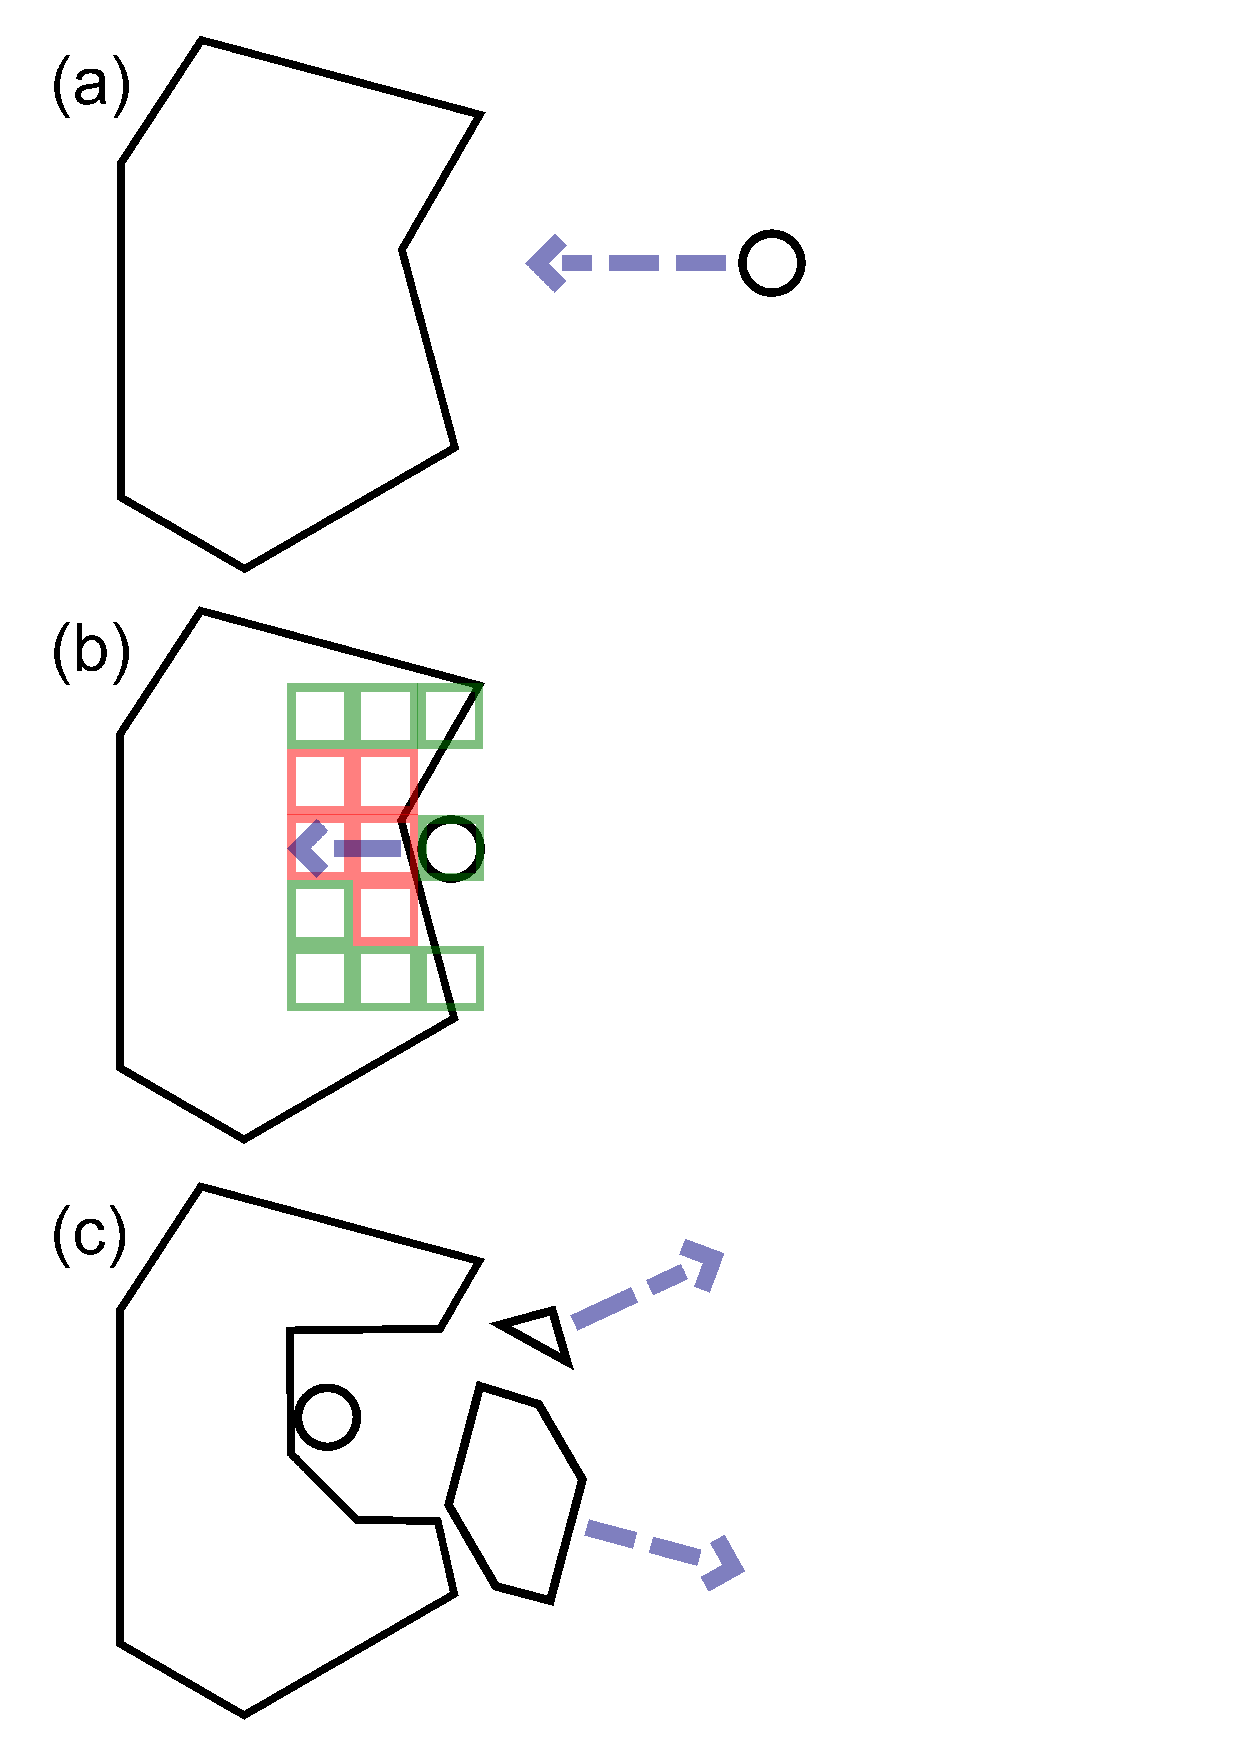
\includegraphics[scale=0.6]{diagram13.pdf}}
\caption{A simple rigid mesh projectile is fired towards another rigid mesh (a). On collision the destructible body is voxelised (b) depending on the force of the projectile and physical parameters of the objects. It is determined which voxels will detach, shown in red. Meshes are reformed around all separate bodies and physical forces are applied (c).}
\label{fig:1.2}
\end{figure}

This process will be referred to as {\emph{Dynamic Volumetric Fragmentation (DVF)}}.

\section{Related Work}

\subsection{Fragmentation}

\label{sect:relfrag}

One existing method for object destruction is a static approach. Fragments are generated for every destructible object when the objects are created and then substituted for the object on collision. This does not allow the result of the collision to be in any way dependant on the forces involved in the collision and so does not produce realistic results.

Matthias M\"{u}ller, Nuttapong Chentanez and Tae-Yong Kim propose a method for the dynamic destruction of objects in real time. The method uses `volume approximate convex decompositions' to fragment objects which are composed of convex pieces using Voronoi decomposition of space\cite{Muller:2013:RTD:2461912.2461934}.

\subsection{Mesh/Voxel Conversion}

Binary voxelisation of polygonal objects is a memory efficient method for defining occupied space and can be achieved in real-time on modern GPUs. Both surface and solid voxelisation methods are presented by Schwarz and Seidel\cite{Schwarz:2010:Vox}. A solid voxelisation algorithm was used as opposed to surface voxelisation as the entire volume of an object is required for the proposed volumetric destruction.

Both marching tetrahedra and surface nets exist as algorithms for constructing 3D surfaces from volumetric data\cite{Tetrahedra}\cite{Gibson:1998:CES:646921.709482}. An existing implementation of marching tetrahedra has been used as part of the remeshing stage of the pipeline as more literature existed concerning the use of this method with Unity3D\cite{Tetrahedra-CPU}.

\subsection{Related Uses}

Nie\ss{}ner et al present a method for real-time collision detection of patch based objects using mesh to voxel transformations \cite{niessner2013collision}. While their work is on collision detection, it does demonstrate that real-time mesh to voxel conversion is viable for use in resolving physics interactions.

Miguel Cepero is developing a procedural voxel engine Voxel Farm\cite{Procedural-World}. His work includes volumetric destruction of objects in a manner similar to this project's aims\cite{Appetite}.


\section{Background}

\subsection{Mesh/Voxel Conversion}

\label{methods}

Binary voxelisation of polygonal objects is a memory efficient method for defining occupied space and can be achieved in real-time on modern GPUs\cite{V,SW,OCL}. I will implement solid voxelisation as opposed to surface volexisation as I require the entire volume of an object to be modelled for my volumetric destruction.

Marching cubes exists as an algorithm for constructing 3D surfaces from volumetric data\cite{MC}. the implementation of this algorithm I will be using runs in real-time on modern GPUs\cite{MCGPU}.

\subsection{Related Work}

Nie\ss{}ner et al present a method for real-time collision detection of patch based objects using mesh to voxel transformations \cite{RTC}. While their work is on collision detection, it does demonstrate that real-time mesh to voxel conversion is viable for use in resolving physics interactions.

Miguel Cepero is developing a procedural voxel engine Voxel Farm\cite{PW}. His work includes volumetric destruction of objects in a manner similar to this project's aims\cite{AfD}.


\section{Methodology}

\subsection{Starting Point}

I will be working using the Unity3D physics and game engine, with which I have prior experience. The engine will provide general features such as rendering, rigid mesh physics and game object management which I will expand upon to achieve my more specific goals. As Unity3D is a widely used commercial engine, its use will also allow for comparable evaluation against scenes implemented using only the base features.

I will be using an existing implementation of the marching cubes algorithm on the GPU for voxel to mesh transformations\cite{MCGPU}.


\subsection{Substance and Structure of the Project}

This project will involve implementing mesh to voxel transformations efficiently at runtime based on existing methods\cite{V,SW,OCL}, as well as the calculation of correct physical responses amongst the individual voxels of the volumetric object. The nature of these physical responses will depend on the physical parameters of the parent object. These parameters and how they impact the physical destruction will have to be defined.

Voxelisation will also be required to be lazy for efficiency. Objects should only be voxelised if the triggering collision is above a certain force threshold which will be defined by the object's physical parameters. If the impact force is not above this then it can be assumed that no damage will be done and there is no need to voxelise. Whole objects should not be voxelised, only a large enough portion to bound the damage that will be done. 

The project has the following main sections:

\begin{enumerate}

\item Real-time voxelization of polygonal meshes on the GPU based on one of the methods cited above.

\item Destruction of volumetric objects based on their physical parameters. By propagating collision information from each voxel to its orthogonal neighbours from the point of impact, it can be calculated which voxels should be dissociated from the parent object and become independent objects.

\item Real-time user modification of objects by adding or removing voxels.

\item Real-time mesh formation from volume data on the GPU using a plugin for Unity3D\cite{MCGPU}.

\item Writing the dissertation.

\end{enumerate}

\clearpage
\subsection{Further goals}

\label{stretch}

If time allows, two further areas will be explored:

\begin{enumerate}

\item \textbf{Object deformation} As well as modelling object destruction while volumetric, object deformation could also be simulated. By representing each voxel as being connected to its neighbours by a rigid bond, the orientation of these bonds can be changed to deform an object based on its malleability, brittleness, density, etc.~.

\item \textbf{Structural integrity.} The main focus of the project is physics caused by interaction such as two objects colliding. A further goal would be modelling the internal physics of resting objects. Take for example a wooden beam fixed at one end with a weight at the other, if this weight is too heavy, the beam should break at the correct point. This simulation is trickier as the cue for when to voxelize and resolve is not as obvious.

\end{enumerate}


\section{Evaluation}

\subsection{Success Criteria}

The following should be achieved:

\begin{itemize}

\item Implement and demonstrate realtime conversion between mesh and volumetric objects.

\item Implement and demonstrate object destruction based on collision information and physical parameters. 

\end{itemize}

\subsection{Evaluation Criteria}

The following are evaluation criteria:

\begin{itemize}

\item A scene with a reasonable number of collisions should run with a framerate above 30FPS and no less than half that of an identical scene using only traditional rigid body physics.
	\begin{itemize}
	\item Comparable scenes built using the base Unity3D rigid mesh physics engine will be used for efficiency evaluation. Metrics to be compared are physics realism, GPU VRAM usage and render thread time.
	\item My own computer will provide a high specification test case, the MCS machines found in the Intel Lab at the William Gates Building will represent a mid range specification.
	\end{itemize}

\item Conversion between mesh and volumetric objects should not be noticeable.
	\begin{itemize}
	\item There should be no obvious slowdown or framerate drop when a conversion occurs.
	\item The delta time between voxelisation and mesh reformation should be below $0.5$s.
	\end{itemize}

\end{itemize}

\subsection{Further Goals}

The following are stretch goals to be achieved if time allows:

\begin{itemize}
\item Volumetric deformation

\item Structural integrity.
\end{itemize}

Further detail can be found in section \ref{stretch}

\clearpage
\subsection{Demonstration}

\label{demo}

At the progress meeting I will demonstrate a stuttered scene in which a bullet will be fired at a brick wall. The scene will be paused at the point of impact for explanation and highlighting of these processes involved:

\begin{enumerate}
\item A portion of the wall and bullet will be voxelised as determined by the force of impact, and the volumetric representations shown as in the video demonstration from Nie{\ss}ner et al\cite{RTCV}.
\item As little progress will have been made on volumetric destruction at this point in the project, instead all the voxels will be removed.
\item The wall's mesh will then be rebuilt from the updated volumetric representation.
\end{enumerate}

A second scene will also be demonstrated in which a ball is dropped from a low height onto another brick wall. It will be shown that no voxelisation takes place as the collision force is not great enough.



\section{Resources}

I will be working with a free license of Unity3D installed on my own computer with the following specifications:
\begin{itemize}
\item 3.40GHz i5-4670k
\item 8GB RAM
\item 400GB remaining SSD storage
\item 750GB remaining HDD storage
\item AMD Radeon HD 7950 GPU
	\begin{itemize}
	\item 3GB GDDR5 Memory
	\end{itemize}
\end{itemize}

I accept full responsibility for this machine and I have made contingency plans to protect myself against hardware and/or software failure.

All source code will be be backed up and version controlled using Git with GitHub. Documentation, as well as any further resources, will be created and stored in a Microsoft OneDrive cloud folder with regular backups to Google Drive as well as my own hard disk drive.



\section{Timeline}

\subsection*{Sprint 1 (24/10/14--7/11/14)}

Implement a mesh to voxel transformation algorithm from section \ref{methods} and become familiar with the voxel to mesh transformation plugin.

Milestones: Some example code, which will probably not be
used in the final project, and some example scenes demonstrating conversion.


\subsection*{Sprint 2 (7/11/14--21/11/14)}

Refactor the mesh to voxel algorithm to only voxelise a portion of an object.

Milestones: Working voxelisation of predefined portions of an object.


\subsection*{Sprint 3 (28/11/14--5/12/14)}

Hook the voxelisation algorithm to collision cues above a predefined threshold.

Milestone: Examples of conversion occurring and not occurring as required on cue.


\subsection*{Sprint 4 (5/12/14--16/1/15)}

Review code and progress over the Christmas break. Ensure everything is well documented, including source and evaluation of current progress.


\subsection*{Sprint 5 (16/1/15--30/1/15)}

Write the initial chapters of the dissertation. Write the progress report. Build the progress demonstration as detailed in section \ref{demo}

Milestones: Preparation chapter of Dissertation complete. Submission of progress report. Demonstration ready.


\subsection*{Sprint 6 (30/1/15--13/2/15)}

Begin to work on physically based destruction algorithms for the splitting apart of volumetric objects, including transferral of force to any objects formed from dissociated voxels. Define the parameters which will impact physical reactions.

Milestones: Ability to define physical properties for game objects.

\clearpage
\subsection*{Sprint 7 (13/2/15--27/2/15)}

Complete work on physically based destruction algorithms.

Milestones: Data confirming impact propagation through voxel bonds.

\subsection*{Sprint 8 (27/2/15--13/3/15)}

Integrate the voxel to mesh plugin with the result of volumetric destruction.

Milestones: Able to see object split apart as the result of an impact of the correct magnitude.


\subsection*{Sprint 9 (13/3/15--27/3/15)}

Implement real-time user modification of objects.

Milestones: Example scene where playing is able to modify objects via physical and non-physical means.


\subsection*{Sprint 10 (27/3/15--10/4/15)}

Code review and code freeze. All success criteria should be implemented by this point. No new features will be written during this period, only bug fixes and optimisations.\\
Further dissertation progress will be made.


\subsection*{Sprint 11 (10/4/15--24/4/15)}

Create comparable scenes using base Unity3D physics for profiling.\\
Profile against these scenes as well as on computers with varying specifications.


\subsection*{Sprint 12 (24/4/15--8/5/15)}

Finish the dissertation, preparing graphs for insertion.  Review the whole
project, check the dissertation, and spend a final few days on
whatever is in greatest need of attention.


\subsection*{Final Sprint (8/5/15--15/5/15)}

Final proofreading and submission of dissertation.

Milestone: Submission of Dissertation. 



\begin{thebibliography}{99}



\bibitem{AfD} Miguel Cepero, (2014), \emph{Appetite for Destruction},\\ Available: http://procworld.blogspot.co.uk/2014/08/appetite-for-destruction.html,\\ Last accessed 22th Oct 2014.

\bibitem{OCL} Miguel Cepero, (2011), \emph{OpenCL Voxelization},\\ Available: http://procworld.blogspot.co.uk/2011/04/opencl-voxelization.html,\\ Last accessed 22th Oct 2014.

\bibitem{PW} Miguel Cepero, (2014), \emph{Procedural World},\\ Available: http://procworld.blogspot.co.uk/,\\ Last accessed 22th Oct 2014.

\bibitem{MCGPU} Scrawk, (2014), \emph{Marching Cubes on the GPU in Unity},\\ Available: http://scrawkblog.com/2014/10/16/marching-cubes-on-the-gpu-in-unity/,\\ Last accessed 22th Oct 2014.

\bibitem{SW} \emph{Fast Parallel Surface and Solid Voxelization on GPUs},\\ M. Schwarz, H. Seidel, \emph{ACM Transactions on Graphics}, Dec 2010, pp.~179:1--179:9.

\bibitem{V} \emph{A Low Cost Antialiased Space Filled Voxelization Of Polygonal Objects
},\\ S. Thon, G. Gesquière, R. Raffin, \emph{Graphicon}, 2004.

\bibitem{MC} \emph{Marching Cubes: A High Resolution 3D Surface Construction Algorithm
},\\ W. Lorensen, H. Cline, \emph{SIGGRAPH Comput. Graph.}, July 1987, pp.~163--169.

\bibitem{RTC} \emph{Real-time Collision Detection for Dynamic Hardware Tessellated Objects
},\\ M. Nie{\ss}ner et al, \emph{Eurographics}, 2013.

\bibitem{RTCV} M. Nie{\ss}ner et al, (2013), \emph{Real-time Collision Detection for Dynamic Hardware Tessellated Objects}, [Online video],\\ Available: \href{http://graphics.stanford.edu/~niessner/papers/2013/2collision/niessner2013collision.mp4}{http://graphics.stanford.edu/$\sim$niessner/papers/2013/}\\\href{http://graphics.stanford.edu/~niessner/papers/2013/2collision/niessner2013collision.mp4}{2collision/niessner2013collision.mp4},\\ Last accessed 23th Oct 2014.

\end{thebibliography}


\end{document}